In this section, we address two key problems outlined in the problem statement (Section 1.2):

\Paragraph{Redundant Work} One significant challenge arises when overlapping or identical range queries are executed in
the database. The conventional approach performs the same amount of work for each query, involving a sort-merge operation 
across multiple levels to filter out invalid keys.

However, a query-driven compaction strategy involves storing the result of the sort-merge operation from the initial 
range query at a higher level. By eliminating invalid keys at an earlier stage, subsequent overlapping range queries 
encounter reduced complexity. This leads to a more efficient execution, as later queries need to read fewer files, 
traverse fewer levels, and consequently encounter fewer invalid keys.

\Paragraph{Increased Write Amplification} The conventional method initiates compactions that retain invalid keys within
the resulting SST files until they reach the last level, thereby causing a rise in write amplification. The query-driven 
compaction strategy helps in eliminating invalid keys throughout the compaction process, resulting in a reduction of 
write amplification and a consequential enhancement in overall system efficiency.

The introduction of aggressive compactions during range queries may create gaps between levels and alter the tree shape. 
Paradoxically, this deformation proves advantageous for future ingestions, acting as a preventive measure against 
triggering cascading compactions.

To substantiate these hypotheses, we conducted a series of experiments on an emulator, implementing the query-driven 
compaction approach. The results validated our expectations, demonstrating that queries following a query-driven 
compaction exhibited significantly improved speed. This optimization not only accelerates query execution but also 
enhances the overall efficiency of the ingestion process.

\Paragraph{Experimental Validation} To provide a more concrete understanding, we implemented the query-driven compaction
approach on RocksDB and conducted a series of experiments to validate its performance in a real-world setting. The 
details of which are outlined below.

\subsection{Experimental Settings}
We ran our experiments on baremetal cloud instances provided by Chameleon. We used `compute skylake' machines to run all 
our experiements.

\begin{itemize}
    \item CPU(s)\:: 48 Cores
    \item RAM\:: 187 GiB
    \item RocksDB version\:: 8.5.0
\end{itemize}

\subsection{Experimental Results}
First set of experiements that we ran were based on our first approach, where each range query has to 
perform query-driven compaction without thinking about the number of entries overlapping between levels. The workload that
we used is as follows.

\begin{enumerate}[leftmargin=*,labelindent=0mm, itemsep=0.2\baselineskip]
    \item Number of Inserts \-- 500000
    \item Number of Updates \-- 250000, 500000, 750000
    \item Number of Range Queries \-- 100 
    \item Selectivity for Range Queries \-- 0.2, 0.4, 0.8
\end{enumerate}

% \begin{figure}
%     \centering
%     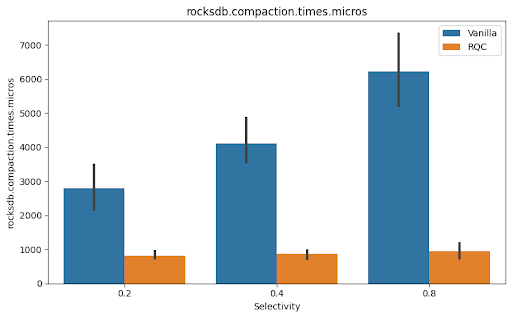
\includegraphics[scale=0.45]{Figures/Compaction Times.png}
%     \caption{Comparison of the number of compactions triggered between RQDC and vanilla. 
%     The results illustrate that RQDC exhibits a significantly lower number of compactions.}\label{fig:compaction_times}
% \end{figure}

% \begin{figure}
%     \centering
%     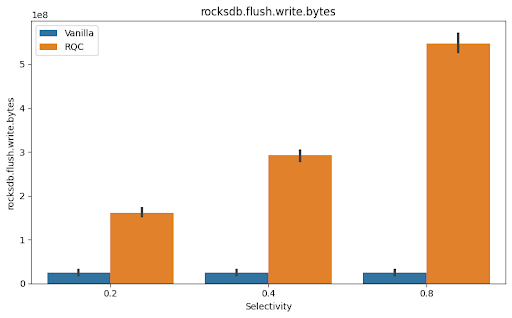
\includegraphics[scale=0.45]{Figures/Range Query Flush Write Bytes.png}
%     \caption{Experiments that shows 10 times more writes with query-driven compaction approach probably because of not 
%     considering the percentage of overlaps between levels}\label{fig:range_query_flush_write_bytes}
% \end{figure}

The results show that the number of compactions triggered during the execution of the entire workload was significantly 
lower in the query-driven compaction than the vanilla approach. This is 
expected since the RQDC approach performed these compactions during the range query executions. Additionally, 
the bytes written during background compactions are comparatively less in RQDC than in vanilla for the same reason. 
The total number of bytes written during the ingestions and the bytes written during the query-driven compaction
is almost 10x higher than the vanilla approach. The positive aspect is that this factor can be tuned by pre-computing 
the overlapping entries between the adjacent levels before performing the range query. If the lower levels have fewer entries 
that overlap with the higher level, then we can perform the vanilla fashion range query. However, if the overlap is more, 
then we can opt for query-driven compaction. These first set of experiments gave us a clear indication that we cannot 
use the query-driven approach for each range query blindly.

% \begin{figure}
%     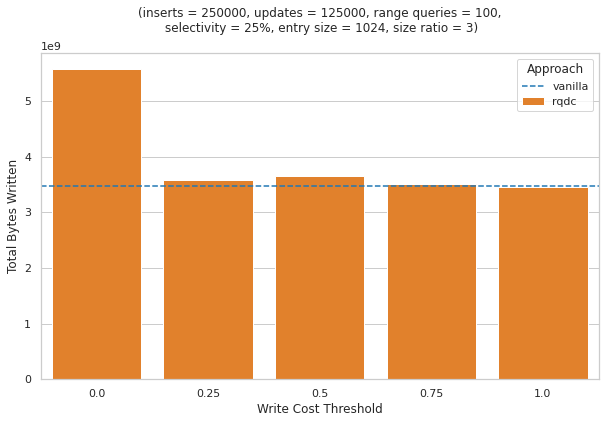
\includegraphics[scale=0.34]{Figures/utl_ltu_approach.png}
%     \caption{Comparison of total write amplification between Vanilla and RQDC using informative compaction approach 
%     (This includes fluhes, compactions, ingestion and RQ writes)}\label{fig:utl_ltu_approach}
% \end{figure}

We ran our second set of experiments using more informative compaction approach that we dicussed in section 4.3. The 
observations are as follows: the new approach has nearly the same write amplification as we have for vanilla and 
it provides a benefit of reduced space amplification. 
% The experiments were conducted several time for a 25\% selectivity 
% of range queries using \textit{lower\_bound} and \textit{upper\_bound} as 0.4 and 0.8 respectively (shown in 
% Figure~\ref{fig:utl_ltu_approach}). The ``Approach-1'' shows the total bytes written for our first approach where it 
% performs compaction for every range query without thinking about the ovalapping entires.
Our third set of experimental design was as follows: we ran each experiment in 11 epochs. The first epoch consisted only 
of inserts, set at 1 million to ensure our database is fully loaded. Subsequently, we ran 10 epochs with each epoch having 
25\% updates and 10 range queries with specific selectivity (10\% results are shown here).The size ratio we choose randomly as 4 \textit{(T)}. 
After each epoch, we recorded the total number of bytes written up to that point, the time taken by each range query for 
that epoch, and the total number of files and keys in our database. 

The Figure~\ref{fig:epoch_experiments} reveals insights into the performance of Vanilla and Query-Driven 
Compaction (RQDC) in this experimental setting. In the Vanilla approach, the total number of files are 1551, containing 
a sum of 1,196,758 entries. In contrast, RQDC demonstrates its efficiency with 982 files and a total of 1,025,110 entries. 
This reduction in the number of files, along with a slightly decreased total entry count comes with a cost 
of more write amplification. 
% This showcases the effectiveness of RQDC in optimizing space utilization.

\begin{figure}
    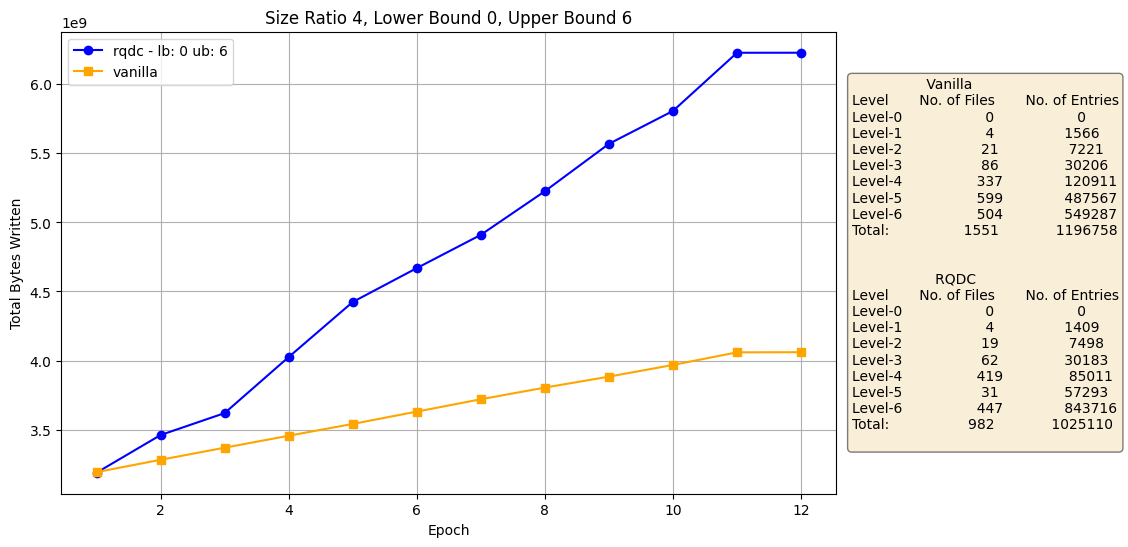
\includegraphics[scale=0.3]{Figures/epoch-experiment-size-ratio-4.png}
    \caption{Results showcasing the trade-off between increased compactions and reduced space amplification. It 
    uses a lower bound of 0 and an upper bound of 6, indicating compactions for nearly every range query to 
    remove possible invalid keys from the tree, unless all range keys exist on a single level.}\label{fig:epoch_experiments}
\end{figure}

\begin{figure}
    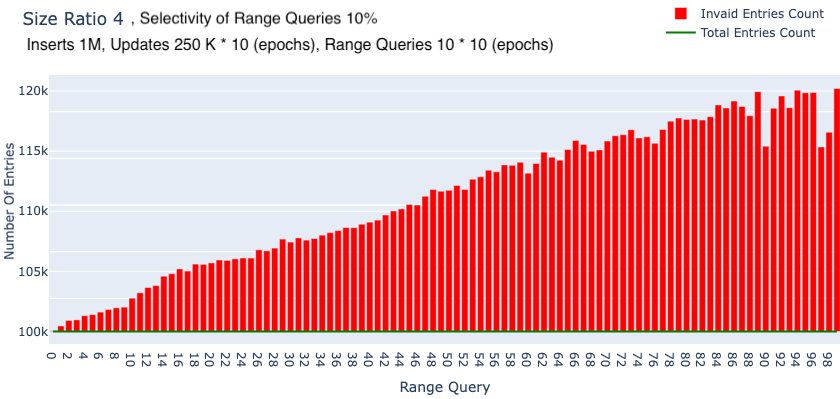
\includegraphics[scale=0.28]{Figures/epoch-experiment-size-ratio-4-vanilla.png}
    \caption{This figure shows the number of invalid entries that were read by range queries during the vanilla 
    workload execution. The horizontal axis represents the range query.}\label{fig:increased_invalid_keys}
\end{figure}

In the vanilla approach, the only mechanism for eliminating invalid keys is through compactions, triggered during newer 
ingestions. In our epoch experiments, we tracked the number of invalid keys that a range query (with a selectivity of 
10\%) had to read from the LSM. We noticed a continuous increase in the count of invalid keys read by range queries, 
reaching up to 2\% of unique inserts by the end of the workload run (depicted in Figure~\ref{fig:increased_invalid_keys}).

% \begin{figure}
%     \centering
    \begin{figure}%{0.45\textwidth}
        \centering
        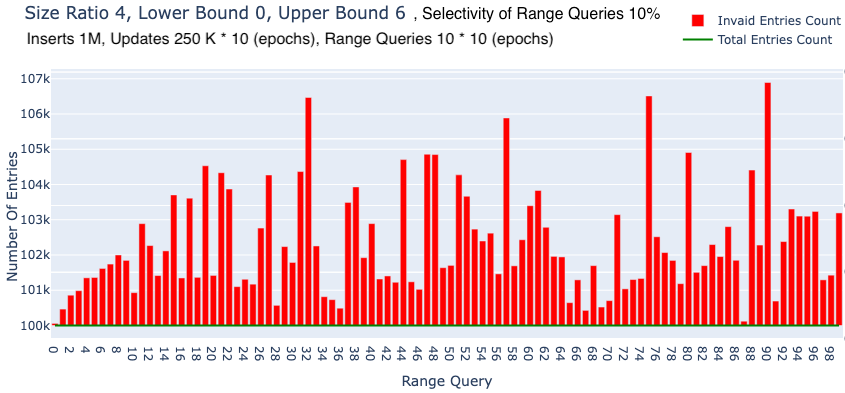
\includegraphics[scale=0.28]{Figures/epoch-experiment-size-ratio-4-range-queries.png}
        \caption{Illustration of the count of invalid entries read by range queries in the RQDC execution for entire the 
        workload, with a lower bound set to 0 and an upper bound set to 6.}\label{fig:reduced_invalid_keys}
    \end{figure}
    \begin{figure}%{0.45\textwidth}
        \centering
        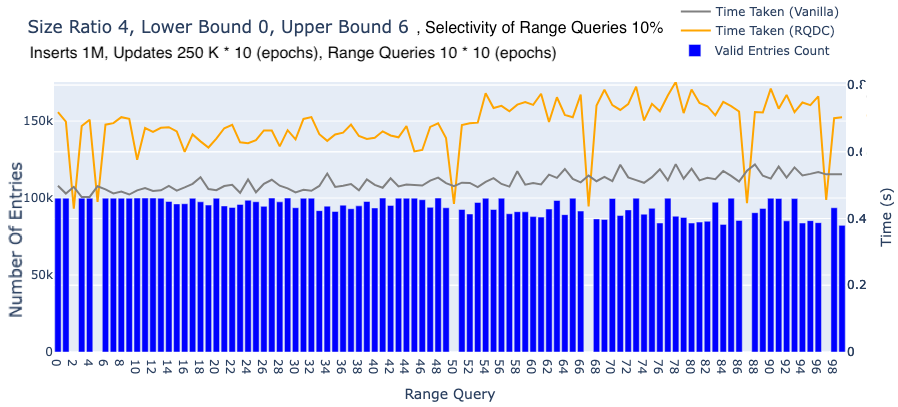
\includegraphics[scale=0.27]{Figures/epoch-experiment-size-ratio-4-rq-time.png}
        \caption{Figure shows the number of entries that were compacted for each range query during the RQDC 
        execution of entire workload. The left vertical axis represent the number of entries that were compacted and right vertical
        axis represent the time taken in seconds by each range query.}\label{fig:increased_range_queries_time}
    \end{figure}
% \end{figure}

When we conducted the same experiment using the RQDC approach, the results were notably different (shown in
Figure~\ref{fig:reduced_invalid_keys}). The maximum number of invalid keys read for a range query was reduced to 0.7\%. 
Although, in comparison to the vanilla approach, the majority of range queries in RQDC retrieved a significantly lower 
number of invalid keys. It's worth noting that this improvement comes at a cost, with approximately a 30\% increase in 
the time required for the execution of a range query (shown in Figure~\ref{fig:increased_range_queries_time}). 
This increase is expected due to the additional writes that RQDC performs during a range query.

We derived a benefit from reduced space amplification, yet the core issues of write amplification and range query 
performance remained unresolved. The \textit{lower\_bound} and \textit{upper\_bound} values we initially employed were 0 
and 6, respectively. These values indicated that whenever a range query had an opportunity to compact, it would do so. 
To address this, we refined the compaction thresholds with the goal of enhancing efficiency. Specifically, we set
a lower threshold of 0.25, indicating that compactions will be suspended for levels where the ratio of entries falling
within the range query is less than 25\% compared to the adjacent next level. Additionally, we set the upper threshold 
to 1.5, signifying that compactions will be halted for levels where the ratio of entries falling within the range query 
exceeds 150\% in comparison to the adjacent next level. These adjustments aim to optimize the compaction process by 
ensuring that the proportion of entries relevant to range queries in each level does not surpass 150\% of the entries 
in the next level.

% \begin{figure}
%     \centering
\begin{figure}%{0.45\textwidth}
    \centering
    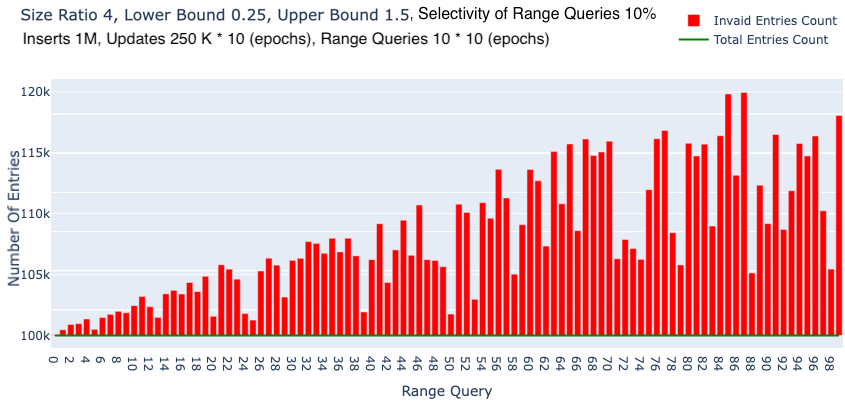
\includegraphics[scale=0.28]{Figures/epoch-experiment-size-ratio-4-lb-ub.png}
    \caption{Shows the number of invalid entries that were read by range queries during the RQDC execution, with a lower bound 
    set to 0.25 and upper bound set to 1.5.}\label{fig:another_epoch_with_lb_ub}
\end{figure}
\begin{figure}%{0.45\textwidth}
    \centering
    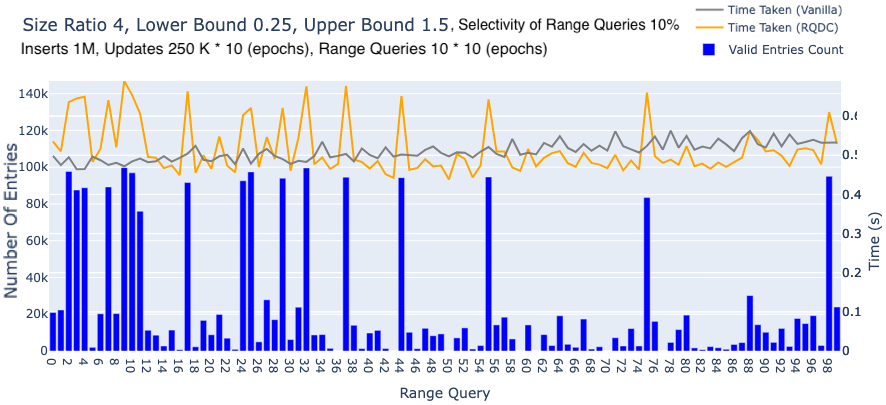
\includegraphics[scale=0.27]{Figures/epoch-experiment-size-ratio-4-rq-time-lb-ub.png}
    \caption{Figure shows the number of entries that were compacted for each range query with time taken during the RQDC 
    with lower bound as 0.25 and upper bound as 1.5.}\label{fig:range_queries_time}
\end{figure}
% \end{figure}

In Figure~\ref{fig:another_epoch_with_lb_ub}, we observe similar trends to those discussed with \textit{lower\_bound} 
set to 0 and \textit{upper\_bound} set to 6. This configuration significantly diminishes the presence of invalid keys to 
the extent that our range queries become more efficient (shown in Figure~\ref{fig:range_queries_time}), although after 
experiencing a minor peaks initially.

The removal of invalid keys during query-driven compaction has a cascading effect on the subsequent range queries 
triggered after a successful execution of the compaction process. In cases where the range is overlapping, these 
subsequent queries read fewer invalid keys, resulting in efficient execution and also solved the challenge 
of performing redundant work.

With the reduction in the presence of invalid keys, a notable improvement is observed. Subsequent executions of the 
same range query are now poised to retrieve only valid keys from the database. This refinement not only optimizes 
query performance but also contributes to a more streamlined and efficient querying process overall.
